\chapter{Adders and Complexity}

\section{Introduction}

Addition is a fundamental part of any ALU and can be easily produced in Verilog by just using ``$+$''.  You will get an adder that is inferred for your FPGA.  The actual adder varies wildly from simple ripple adders, to specialized pre-built hardware blocks.  We are going to explicitly build three different adders with very different complexities and compare them.

\subsection{Ripple Adders}

This is the technique that is covered in digital logic.  Basically, full bit adders, see Figure~\ref{f-half_full_add}, are created and cascaded together.  The carry bit from the previous full adder must arrive before the result is added.  The resulting valid carries thus ripple down to the most significant bit (hence the name).  Adding $n$ bit numbers, thus takes the propagation time of $n+1$ levels of logic, i.e. it is O(n) in time to calculate addition.  Thus if 32 bit numbers are added on fast logic (1ns per stage/gate) the process would take 33ns.  This is way too slow.  On the bright side, none of the gates take more than 2 inputs so the size of the gates is O(1).

\begin{figure}
\caption{(left) Half Adder, (right) Full Adder}\label{f-half_full_add}
\begin{center}
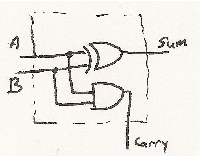
\includegraphics{ha.png} \hspace{.2in} 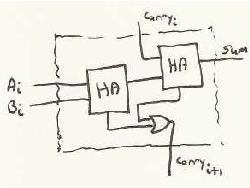
\includegraphics{fa.png}
\end{center}
\end{figure}

\subsection{Conditional Sum}
Conditional sum is a divide and conquer algorithm, and hence exploits binary tree parallelism.  The algorithm works by calculating both possible results for each bit (if carry in was 1 or 0), then performing paired conditional concatenation using the actual carry bit of the lower number, see Figure~\ref{f-cond_sum_add}.

\begin{figure}
\caption{Conditional Sum Adder (above), and its sub-blocks (below, left and right).}\label{f-cond_sum_add}
\begin{center}
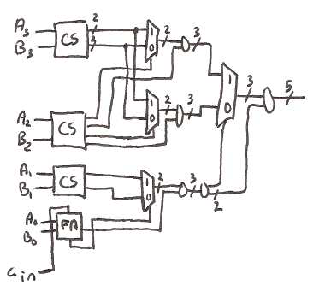
\includegraphics{conditional_sum.png}\\\vspace{.2in}
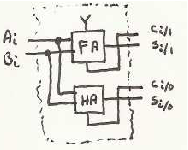
\includegraphics{cs_4out.png} \hspace{.2in} 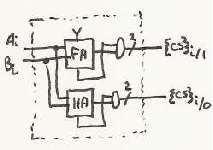
\includegraphics{cs_2out.png}
\end{center}
\end{figure}

\begin{enumerate}
    \item form conditional terms for each digit in summation $\rightarrow$ (digit with carry, digit without carry) = ($x_i+y_i+1$,$x_i+y_i$)
    \item group by twos from right and for both conditional values in the right parenthesis form the result as follows:
    \begin{enumerate}
        \item the leftmost bit of the two terms on the right are the carry bits used to select the term on the left
        \item concatenate the appropriate term on the left (picked by carry) with each term on right after removing the parity bits of the right terms
    \end{enumerate}
    \item continue pairings until only 1 term remains. pick right number if $c_{in}=0$ else pick left.
\end{enumerate}

\begin{example}
 Add $x=0110$ and $y=1111$ by conditional sum and indicate if overflow occurred.

        {\color{ans}
        \begin{tabular}{cccc}
          0+1 & 1+1 & 1+1 & 0+1 \\
          $\downarrow$ & $\downarrow$ & $\downarrow$ & $\downarrow$ \\
          (10,01) & (11,10) & (11,10) & (10,01) \\
          $\searrow$ & $\swarrow$ & $\searrow$ & $\swarrow$ \\
          \multicolumn{2}{r}{(101,100} & \multicolumn{2}{l}{(110,101)} \\
          \multicolumn{2}{c}{$\searrow$} & \multicolumn{2}{c}{$\swarrow$} \\
          \multicolumn{4}{c}{(10110,10101)} \\
          \multicolumn{4}{c}{1 0101} \\
        \end{tabular}

        No overflow occurred (added a positive and negative number).
        }
\end{example}



\begin{example}
    Calculate $7-8$ by conditional sum.

    {\color{ans}

    $7=0111$ and $-8=1000$

    \begin{tabular}{cccc}
    $\;$ 0       & 1          & 1          & 1          \\
      +1         & 0          & 0          & 0          \\ \hline
      (10,01)    & (10,01)    & (10,01)    & (10,01)    \\
      $\searrow$ & $\swarrow$ & $\searrow$ & $\swarrow$ \\
      \multicolumn{2}{c}{(100,011)} & \multicolumn{2}{c}{(100,011)} \\
      \multicolumn{2}{c}{$\quad\searrow$} & \multicolumn{2}{c}{$\swarrow\quad$} \\
      \multicolumn{4}{c}{(10000,01111)} \\
    \end{tabular}

    Since this was done as addition no carry-in was set so the solution is \begin{tabular}{r|l} 0 & 1111 \\ \hline \end{tabular} or $-1$ in signed base ten.

    }
\end{example}


\begin{example}
Add by conditional sum $x=01100110$ and $y=00110011$.

{\color{ans}
\noindent
\begin{tabular}{rrrrrrrr}
$0+0$ & $1+0$ & $1+1$ & $0+1$ & $0+0$ & $1+0$ & $1+1$ & $0+1$ \\
$\downarrow$ & $\downarrow$ & $\downarrow$ & $\downarrow$ & $\downarrow$ & $\downarrow$ & $\downarrow$ & $\downarrow$ \\
$(01,00)$ & $(10,01)$ & $(11,10)$ & $(10,01)$ & $(01,00)$ & $(10,01)$ & $(11,10)$ & $(10,01)$ \\
$\searrow$ & $\downarrow$ & $\searrow$ & $\downarrow$ & $\searrow$ & $\downarrow$ & $\searrow$ & $\downarrow$ \\
\multicolumn{2}{r}{$(010,001)$} & \multicolumn{2}{r}{$(110,101)$} & \multicolumn{2}{r}{$(010,001)$} & \multicolumn{2}{r}{$(110,101)$} \\
& $\searrow$ & & $\swarrow$ & & $\searrow$ & & $\swarrow$  \\
&  & \multicolumn{2}{c}{$(01010,01001)$} &  &  & \multicolumn{2}{c}{$(01010,01001)$ }  \\
&  &  & $\searrow$ &  & $\swarrow$ &  &  \\
&  &  & \multicolumn{3}{c}{$(010011010,010011001)$} &  &  \\
&  &  & \multicolumn{3}{c}{$0 \, 10011001$} &  &  \\
\end{tabular}
}
\end{example}

Why go through this?  First, by a folk theorem of Dr. Alan Laub, ``\emph{What is hard for us tends to be easy for computers (and vice versa)}.''  In reality this process is really easy for a computer to do.  Second, the process is highly parallel, so it can be done very fast.  If the numbers to be added are n bits long this takes $2(\log_2(n)+1)$ levels of logic, much better than the $n+1$ levels of logic required by ripple calculations.  Thus it is O(log(n)) in time complexity.  For example, for adding the 32 bit numbers considered already, conditional sum would take $2(\log_2(32)+1)=12$ levels of logic, so on the fast logic described it would be 12ns, a huge improvement.

\subsection{Carry-Lookahead}

This is also referred to as lookahead carry.  Assume $x+y=z$.  Pre-generate all carries with 2-level logic. Usually form (g,p,c) generate, propagate, carry.
\begin{eqnarray}
G_i & = & x_i \cdot y_i \\
P_i & = & x_i + y_i \\
C_i & = & G_i + P_i \cdot C_{i-1} \\
    & = & G_i + P_i \cdot (G_{i-1} + P_{i-1} \cdot C_{i-2}) \\
    & = & G_i + P_i \cdot G_{i-1} + P_i \cdot P_{i-1} \cdot C_{i-2} \\
    & = & G_i + P_i \cdot G_{i-1} + P_i \cdot P_{i-1} \cdot G_{i-2} +
    \ldots + P_i \cdot P_{i-1} \cdot \ldots \cdot P_0 \cdot C_{in}
\end{eqnarray}

This method is very fast (regardless of size it take 5 levels of logic) but requires large gates for problems of reasonable size (even 16 or 32 bit numbers) and thus has problems with fan-in, fan-out, and size.

Often blocks of a number are handled with lookahead, and the blocks are connected in some fashion (for example ripple) to get the net result (i.e. just like single bit adds from a full adder are connected to propagate the carry bit, blocks or 4, 8, or more could be handled lookahead then connected to propagate the carry bit between them to handle a larger number, say 32 bits).  Even better than cascading (ripple connection) the adders, is to us group carry-lookahead, in which each of the carry-lookahead adders output their group propagate and group generate variables to a circuit that generates the carry-in bits for each group.  It takes 5 logic levels to generate the carries to each individual carry-lookahead adder, and each adder then takes 5 levels of logic to get the result, for a total of 10 levels of logic.  For the example of adding 32 bit numbers with fast logic, it would take 10ns with group carry-lookahead adders (probably four or eight bits in a group).


\begin{example}
Specify the equations of a two bit binary adder with carry in (i.e.: one equation for each of the sum bits and one equation for the carry out).  Put the equations in sum of products form.

{\color{ans}Sol:
Let the two numbers to be added be $A_1 A_0$ and $B_1 B_0$.  Let the resulting sum be $S_1 S_0$.  Let the carries be $C_{in}$ and $C_{out}$.  Finally, let $C_0$ be the carry from the first bit added (saves writing).
\begin{eqnarray}
S_0 & = & A_0 \oplus B_0 \oplus C_{in} \\
C_0 & = & A_0\cdot B_0 + A_0\cdot C_{in} + B_0\cdot C_{in} \\
S_1 & = & A_1 \oplus B_1 \oplus C_0\\
C_{out} & = & A_1 \cdot B_1 + A_1 \cdot C_0 + B_1 \cdot C_0
\end{eqnarray}
Putting this in sum of products form yields
\begin{eqnarray}
S_0 & = & A_0' \cdot B_0' \cdot C_{in} +
          A_0' \cdot B_0 \cdot C_{in}' +
          A_0 \cdot B_0' \cdot C_{in}' +
          A_0 \cdot B_0 \cdot C_{in} \\
S_1 & = & A_1' \cdot B_1' \cdot (A_0\cdot B_0 + A_0\cdot C_{in} + B_0\cdot C_{in}) +
          A_1' \cdot B_1 \cdot (A_0\cdot B_0 + A_0\cdot C_{in} + B_0\cdot C_{in})' + \\
    & & \qquad A_1 \cdot B_1' \cdot (A_0\cdot B_0 + A_0\cdot C_{in} + B_0\cdot C_{in})' +
          A_1 \cdot B_1 \cdot (A_0\cdot B_0 + A_0\cdot C_{in} + B_0\cdot C_{in}) \\
    & = & A_1' \cdot B_1' \cdot A_0\cdot B_0 + A_1' \cdot B_1' \cdot A_0 \cdot C_{in}
          + A_1' \cdot B_1' \cdot B_0\cdot C_{in} \\
    & & \qquad
          + A_1' \cdot B_1 \cdot (A_0'\cdot B_0' + A_0'\cdot C_{in}' + B_0'\cdot C_{in}') \\
    & & \qquad
          + A_1 \cdot B_1' \cdot (A_0'\cdot B_0' + A_0'\cdot C_{in}' + B_0'\cdot C_{in}') \\
    & & \qquad
          + A_1 \cdot B_1 \cdot A_0\cdot B_0 + A_1 \cdot B_1 \cdot A_0\cdot C_{in}
           + A_1 \cdot B_1 \cdot B_0\cdot C_{in} \\
    & = & A_1' \cdot B_1' \cdot A_0\cdot B_0 + A_1' \cdot B_1' \cdot A_0 \cdot C_{in}
          + A_1' \cdot B_1' \cdot B_0\cdot C_{in} \\
    & & \qquad
          + A_1' \cdot B_1 \cdot A_0'\cdot B_0' + A_1' \cdot B_1 \cdot A_0'\cdot C_{in}'
          + A_1' \cdot B_1 \cdot B_0'\cdot C_{in}' \\
    & & \qquad
          + A_1 \cdot B_1' \cdot A_0'\cdot B_0' + A_1 \cdot B_1' \cdot A_0'\cdot C_{in}'
          + A_1 \cdot B_1' \cdot B_0'\cdot C_{in}' \\
    & & \qquad
          + A_1 \cdot B_1 \cdot A_0\cdot B_0 + A_1 \cdot B_1 \cdot A_0\cdot C_{in}
           + A_1 \cdot B_1 \cdot B_0\cdot C_{in} \\
C_{out} & = & A_1 \cdot B_1 + A_1 \cdot (A_0\cdot B_0 + A_0\cdot C_{in} + B_0\cdot C_{in}) \\
   & & \qquad + B_1 \cdot (A_0\cdot B_0 + A_0\cdot C_{in} + B_0\cdot C_{in}) \\
    & = & A_1 \cdot B_1 + A_1 \cdot A_0\cdot B_0 + A_1 \cdot A_0\cdot C_{in} + A_1 \cdot B_0\cdot C_{in} \\
   & & \qquad + B_1 \cdot A_0\cdot B_0 + B_1 \cdot A_0\cdot C_{in} + B_1 \cdot B_0\cdot C_{in}
\end{eqnarray}
}
\end{example}

\section{Generate}

The Verilog generate command is a powerful tool.  Consider the code to generate a ripple carry adder below.
\Code{Ripple adder}{ra}{../code/adder/ripple.v}{verilog}



\section{Assignment}

Build 8-bit adders for:
\begin{enumerate}
\item ripple carry adder
\item conditional sum adder
\item block carry lookahead, with 4-bit blocks
\end{enumerate}